\chapter{Relations et opérations fondamentales dans l'ensemble des nombres décimaux et des fractions.}

{\AlegreyaSansLight \large
\begin{center}
\textbf{Crédit :} 32 heures\\
\textit{4 heures hebdomadaires}
\end{center}
}

\minitoc

\section{Introduction}
\subsection{Présentation du module}
Ce module vise à rendre l'apprenant capable de traiter de façon réussie, des situations de vie de la famille "représentation, détermination des quantités et identification des objets par des nombres ". Il s'agit en gros, de le rendre capable de :
\begin{itemize}
\item Résoudre des problèmes relatifs à des situations de vie telles que : l'achat ou la vente des biens de consommation, le partage des biens, la vérification d'une facture après payement la comparaison des prix des objets …
\item Communiquer des informations comportant des nombres (numéros de téléphones, matricule, immatriculation d'un véhicule …);
\end{itemize}
Il importe pour cela de consolider les notions d'addition, de soustraction, de multiplication de division et de relation d'ordre vues en 6ème. Les savoirs essentiels associés au présent module constituent cependant une avancée vers une habileté cognitive supérieure en l'occurrence l'application (division euclidienne, décomposition
d'un entier en produit de facteurs premiers, résolution des équations, etc.). L'enseignant pourra donc mettre un accent sur cette habileté dans les compétences liées à la résolution des problèmes.

\subsection{Contribution du module à la finalité et aux buts curriculaires}
Ce module permet de développer les compétences transversales suivantes : l'esprit critique, le sens de l'ordre et de la méthode, le sens de la rigueur et de la concision, le sens de la prévision et de l'estimation. Il contribue au renforcement de la pratique du calcul mental, à l'utilisation de la calculatrice ; ce qui permet à l'apprenant d'agir de manière autonome, compétente et adaptative dans diverses situations de la vie courante, dans lesquelles ces pratiques interviennent.

\subsection{Contribution du module au programme d'études et aux domaines de vie}
Ce module qui fait partie des programmes de mathématiques permet à chaque apprenant d'acquérir des connaissances et savoir-faire de base sur lesquels les enseignements/apprentissages qu'il recevra dans les autres disciplines du domaine d'apprentissage devront s'appuyer.\\
Les nombres décimaux sont utilisés dans toutes les sciences pour mesurer, peser et évaluer les quantités.\\
La maîtrise des concepts d'égalité, d'inégalité et des opérations fondamentales que sont l'addition, la soustraction, la multiplication et la division, est de nature à doter l'apprenant d'un certain nombre d' outils fondamentaux dont il aura besoin dans la vie pratique.\\
La gestion du budget familial, la comptabilité au sein de l'entreprise, l'évaluation des distances, des poids, des volumes, sont autant d'applications des nombres décimaux dans les domaines de vie que sont l'économie, les média, l'environnement, la santé et le bien être.

\section{Matrice}

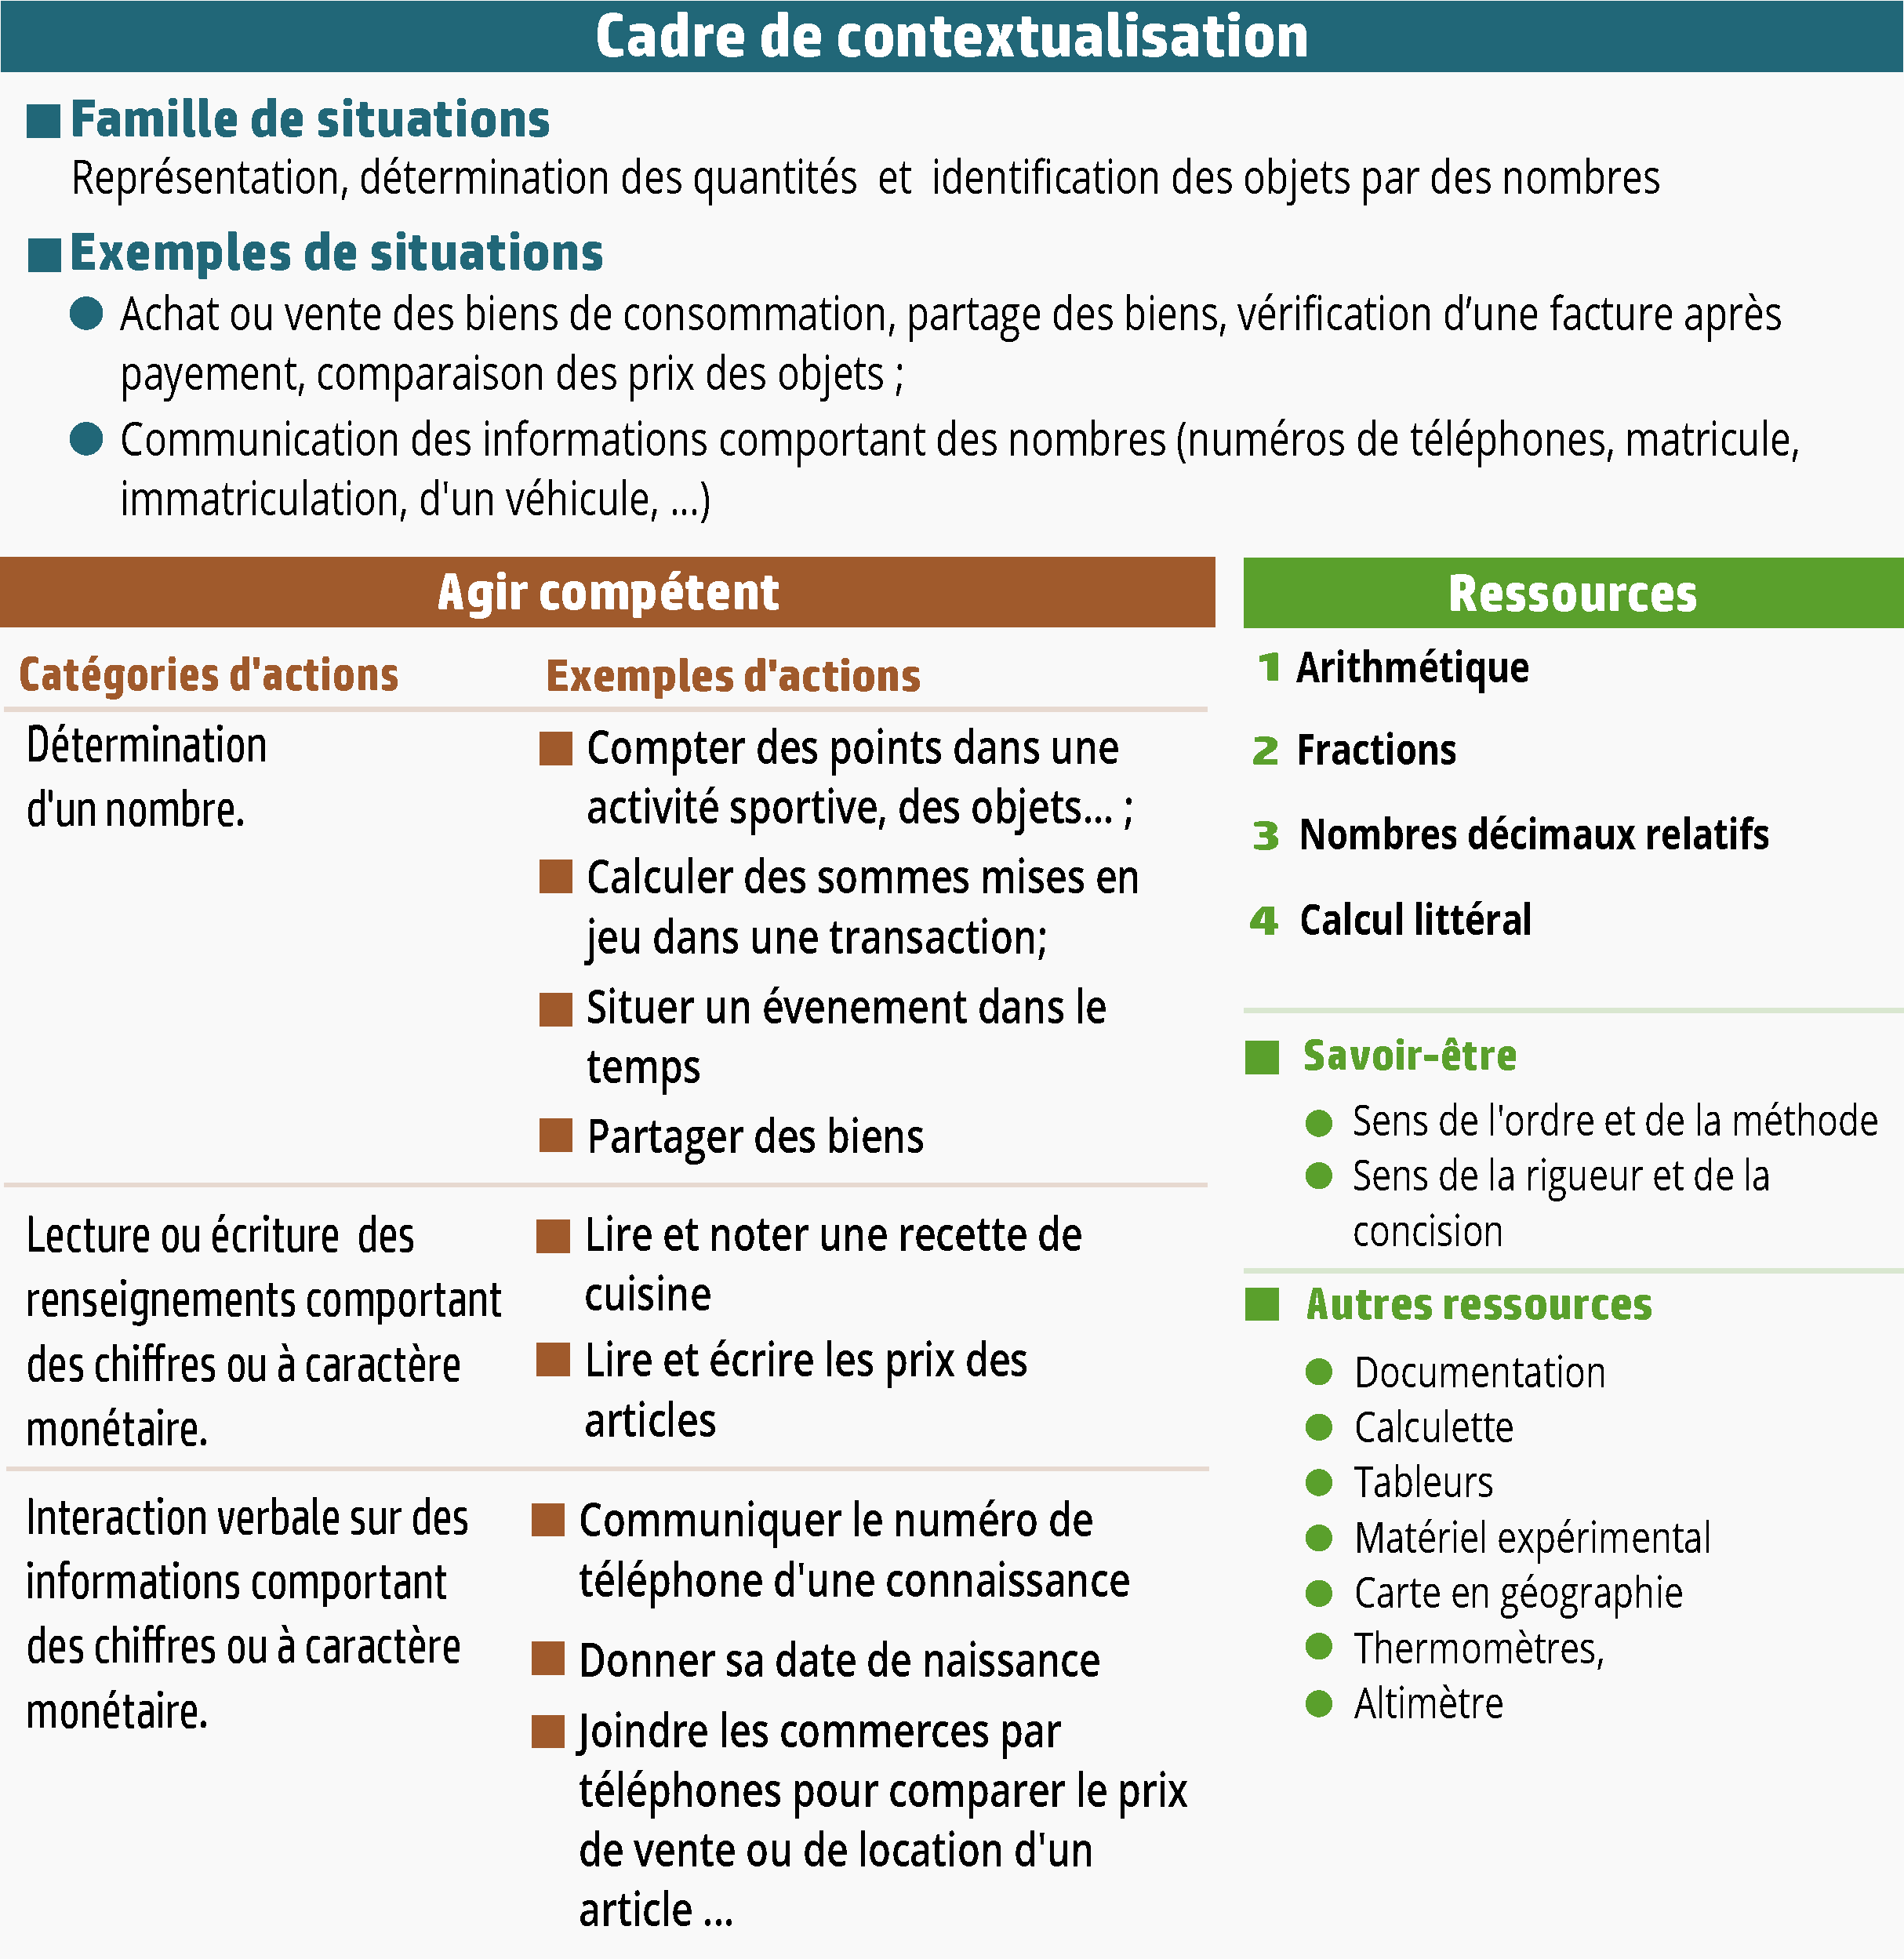
\includegraphics[width=\textwidth]{Module5.pdf} 

\subsection*{}
\addcontentsline{toc}{subsection}{\textbf{Ressource 1}: arithmétique}
\ressource{Ari.pdf}

\savoir
\begin{itemize}
\item Division euclidienne ;
\item Puissance entière d'un entier naturel ;
\item Nombres premiers ;
\item PPMC et PGDC.
\end{itemize}
\savoirfaire
\begin{itemize}
\item Décomposition en produit de facteurs premiers ;
\item Application à la recherche des multiples ou des diviseurs ;
\item Calcul du PPMC et PGDC ;
\item Critère de divisibilité : par 4 et 25.
\end{itemize}

\subsection*{}
\addcontentsline{toc}{subsection}{\textbf{Ressource 2}: fractions}
\ressource{Fractions.pdf}

\savoir
\begin{itemize}
\item Fractions irréductibles
\end{itemize}
\savoirfaire
\begin{itemize}
\item Comparaison des fractions.
\item Encadrement des fractions par deux nombres décimaux de même ordre (consécutifs) ;
\item Somme, différence, produit, division de fractions.
\end{itemize}

\subsection*{}
\addcontentsline{toc}{subsection}{\textbf{Ressource 3}: nombres décimaux relatifs}
\ressource{D5.pdf}

\savoir
\begin{itemize}
\item Opposé d'un nombre décimal relatif.
\item Puissance d'un nombre décimal relatif à exposant entier naturel non nul.
\end{itemize}
\savoirfaire
\begin{itemize}
\item Addition, soustraction, multiplication et division des nombres décimaux;
\item Calculs sur les puissances ;
\item Comparaison des nombres décimaux relatifs.
\end{itemize}

\subsection*{}
\addcontentsline{toc}{subsection}{\textbf{Ressource 4}: calcul littéral}
\ressource{CL5.pdf}

\savoir

\textbf{Equations du type:}
\begin{itemize}
\item  $a+x=b$ dans $\G D$;
\item $ax=b$ où $a$ et $b$ sont des entiers, $a$ non nul.
\end{itemize}